% This work is licensed under the Creative Commons
% Attribution-NonCommercial 3.0 Unported License. To view a copy of this
% license, visit http://creativecommons.org/licenses/by-nc/3.0/.

\section{Durchführung}
In diesem Versuch werden ein RLC-Kreis, ein Funktionsgenerator, ein
Oszilloskop und ein Voltmeter verwendet. Der RLC-Kreis trägt die
Aufschrift \enquote{Gerät 2}.  Ein schematischer Aufbau des Versuches
ist in Abb. \ref{fig:aufbau} zu sehen.

Der in dieser Abbildung zu sehende Schalter ist im wirklichen
Versuchsaufbau nicht vorhanden. Der Schalter symbolisiert nur die
Tatsache, dass die Kondensatorspannung des RLC-Kreises in diesem Versuch
für verschiedene Messungen entweder mit einem Oszilloskopen oder mit
einem Voltmeter abgegriffen wird.
%
\begin{figure}
\centering
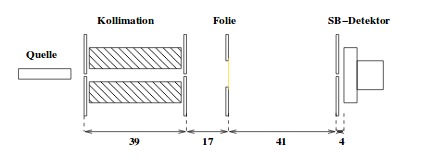
\includegraphics[width=0.7\textwidth]{aufbau}
\caption{Skizze der verwendeten Versuchsapparatur}
\label{fig:aufbau}
\end{figure}
%

Als erstes werden die gedämpften Schwingungen untersucht. Dazu wird
mithilfe des Funktionsgenerators eine Rechteckspannung generiert, die
eine solche niedrige Frequenz besitzt, dass der RLC-Kreis während einer
halben Periode der Rechteckspannung mehrere gedämpfte Schwingungen
durchführen kann.  Diese Schwingungen werden auf einem Oszilloskop
betrachtet und das getriggerte Bild gespeichert.  In diesem Versuchsteil
wird der Widerstand $R_1$ des RLC-Kreises verwendet.

Im nächsten Schritt soll der Dämpfungswiderstand $R_\text{ap}$ des
aperiodischen Grenzfalls bestimmt werden. Dazu wird ein regelbarer
Widerstand anstelle des Widerstandes $R_1$ in den RLC-Kreis
eingebaut. Dieser wird zunächst auf seinen Maximalwert eingestellt. Der
Funktionsgenerator generiert immernoch Rechteckspannungen und die
Kondensatorspannung wird auf dem Oszilloskopen betrachetet.  Nun wird
der regelbare Widerstand so lange erniedrigt, bis sich der aperiodische
Abfall der Kondensatorspannung zeigt. Diesen erkennt man daran, dass bei
leichter Erhöhung des Widerstandes ein Unterschwingen eintritt.

Als nächstes wird die Frequenzabhängigkeit der Amplitudenspannung des
Kondensators analysiert. Dazu wird eine Sinusspannung vom
Funktionsgenerator generiert und wieder der Widerstand $R_1$ in den
RLC-Kreis eingebaut.  Diesmal wird die Kondensatorspannung $U_\text{C}$
mit einem AC-Millivoltmeter abgegriffen. Es wird eine Messreihe
erstellt, in der zu 51 Frequenzen von \SI{10}{\kilo\hertz} bis
\SI{50}{\kilo\hertz} die Kondensatorspannungen gemessen werden.

Als letztes wird noch eine Messreihe zur Untersuchung der
Frequenzabhängigkeit des Phasenunterschiedes zwischen Erreger- und
Kondensatorspannung durchgeführt.  Hierbei wird die Kondensatorspannung
und die Erregerspannung mit dem Oszilloskop gleichzeitig betrachtet und
der Funktionsgenerator liefert eine Sinusspannung.  Der interne
Widerstand des RLC-Kreises wird nun auf den Widerstand mit der
Aufschrift $R_2$ gewechselt.  In der letzten Messreihe werden zu 16
Frequenzen zwischen \SI{10}{\kilo\hertz} und \SI{32.5}{\kilo\hertz} die
Zeitdifferenzen $\Delta t$ zwischen den Nulldurchläufen von Erreger- und
Kondensatorspannung gemessen. Dazu werden die Spannungskurven der beiden
Spannungen symmetrisch um die Zeitachse gelegt und die Zeitdifferenz der
Nulldurchgänge anschließend mithilfe der Cursors des Oszilloskops
vermessen.
